\documentclass[11pt,aspectratio=169]{beamer}

% =========================================================
% FONTS & PACKAGES -- styled after /Users/xiaohao/thesis/thesis_talk/talk.tex
% =========================================================
\usepackage[T1]{fontenc}
\usepackage{newpxtext}
\usepackage{fontawesome5}
\usepackage{xcolor}
\usepackage{amsmath,amssymb,mathtools}
\usepackage{mathrsfs}
\usepackage{tikz}
\usepackage{graphicx}
\usepackage{booktabs}
\usepackage{tabularx}
\usepackage{array}
\usepackage{multicol}
\usetikzlibrary{positioning,arrows.meta,fit,calc}

\graphicspath{{../demo/build/results/figures/}{fig/}}

% =========================================================
% COLORS
% =========================================================
\definecolor{midnightblue}{RGB}{25, 25, 112}
\definecolor{pinegreen}{RGB}{1, 121, 111}
\definecolor{grayline}{RGB}{180, 180, 180}
\definecolor{graygreen}{RGB}{85, 120, 105}
\definecolor{midnightblueLight}{RGB}{100, 149, 237}
\definecolor{fuBlue}{RGB}{0,51,102}
\definecolor{warmgray}{RGB}{245,244,241}

% =========================================================
% LOCAL MACROS
% =========================================================
\newcommand{\dd}{\,\mathrm{d}}
\newcommand{\E}{\mathbb{E}}
\newcommand{\R}{\mathbb{R}}
\newcommand{\1}{\mathbf{1}}
\newcommand{\mcl}{\mathcal}
\newcommand{\BS}{Black--Scholes}
\newcommand{\BSDE}{BSDE}
\newcommand{\LRH}{Lifted Rough Heston}
\newcommand{\VRP}{\mathrm{VRP}}
\newcommand{\PnL}{P\&L}
\newcommand{\talkcite}[1]{{\scriptsize\color{graygreen}\cite{#1}}}
\newcommand{\claim}[1]{\textcolor{midnightblue}{\textbf{#1}}}

% =========================================================
% BEAMER THEME SETTINGS
% =========================================================
\mode<presentation>{
    \usetheme{Boadilla}
    \usecolortheme{default}
    \usefonttheme{serif}

    \setbeamercolor{structure}{fg=midnightblue}
    \setbeamercolor{title}{fg=midnightblue}
    \setbeamercolor{frametitle}{fg=midnightblue}
    \setbeamercolor{normal text}{fg=black,bg=white}
    \setbeamercolor{itemize item}{fg=midnightblue}
    \setbeamercolor{itemize subitem}{fg=midnightblueLight}
    \setbeamertemplate{itemize items}[circle]
    \setbeamertemplate{enumerate items}[default]
    \setbeamercolor{block title}{bg=midnightblue, fg=white}
    \setbeamercolor{block body}{bg=midnightblue!5, fg=black}
    \setbeamercolor{block title alerted}{bg=pinegreen, fg=white}
    \setbeamercolor{block body alerted}{bg=pinegreen!6, fg=black}
    \setbeamertemplate{navigation symbols}{}
}
\setbeamertemplate{bibliography item}{\insertbiblabel}
\setbeamerfont{footnote}{size=\tiny}
\setbeamerfont{caption}{size=\scriptsize}

% =========================================================
% HYPERLINKS
% =========================================================
\hypersetup{
    colorlinks=true,
    linkcolor=midnightblue,
    citecolor=midnightblue,
    urlcolor=pinegreen,
}
\pdfstringdefDisableCommands{\def\\{ }}

% =========================================================
% TITLE PAGE INFORMATION
% =========================================================
\title[Effective Engine MVP]{Effective Engine MVP}
\subtitle{Variance alpha, neural BSDE hedging, and execution-aware walk-forward retraining}
\author[X. Ji]{\textbf{Xiaohao Ji}}
\institute[Independent Project]{
    Project report -- 30--45 minutes\\[4pt]
    C++ options trading engine + Python research pipeline
}
\date{2026}

% =========================================================
% SECTION SLIDES
% =========================================================
\AtBeginSection[]{
  \begin{frame}
    \vfill
    \centering
    \begin{beamercolorbox}[sep=8pt,center,shadow=true,rounded=true]{title}
      \usebeamerfont{title}\insertsectionhead\par%
    \end{beamercolorbox}
    \vfill
  \end{frame}
}

\begin{document}

\begin{frame}
    \titlepage
\end{frame}

\begin{frame}{Thirty-Five Minute Map}
    \scriptsize
    \begin{center}
    \begin{tabular}{p{0.22\textwidth}p{0.58\textwidth}p{0.11\textwidth}}
        \toprule
        \textbf{Part} & \textbf{Main message} & \textbf{Time} \\
        \midrule
        Motivation & Options alpha is signal, hedge, execution, and validation. & 5 min \\
        State of art & From \BS{} to rough vol and deep hedging; deployment remains hard. & 7 min \\
        Core idea & Use BSDE learning as a hedge operator, not an alpha destroyer. & 10 min \\
        System & C++ replay plus Python walk-forward retraining makes the idea testable. & 8 min \\
        Results & Delta-only BSDE preserves most of BS Delta's OOS VRP capture. & 7 min \\
        Outlook & Mature pieces, research-grade pieces, and next steps. & 3 min \\
        \bottomrule
    \end{tabular}
    \end{center}
    \vspace{2pt}
    \begin{block}{Talk spine}
    A research prototype for equity-index volatility trading: choose the right hedge objective, replay honestly, and promote only after walk-forward gates.
    \end{block}
\end{frame}

\begin{frame}{The Project In One Picture}
\centering
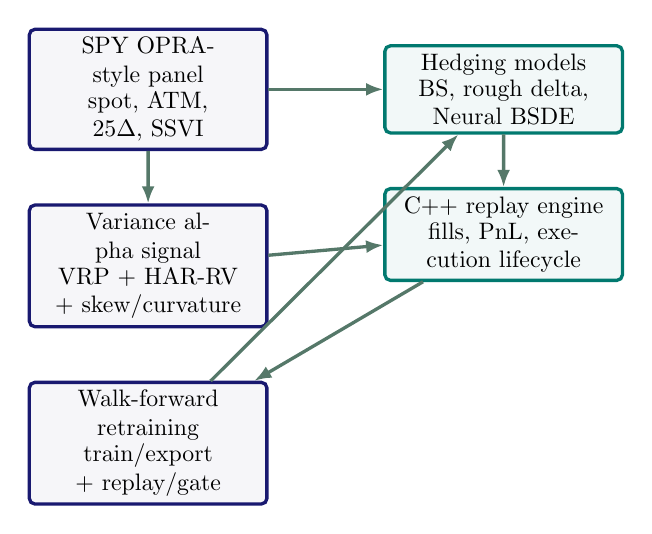
\begin{tikzpicture}[
    scale=0.86,
    transform shape,
    node distance=0.78cm,
    box/.style={draw=midnightblue, rounded corners=2pt, very thick, align=center,
        minimum height=0.74cm, text width=0.27\textwidth, fill=midnightblue!4},
    gbox/.style={draw=pinegreen, rounded corners=2pt, very thick, align=center,
        minimum height=0.74cm, text width=0.27\textwidth, fill=pinegreen!5},
    arrow/.style={-{Latex[length=2.2mm]}, very thick, draw=graygreen}
]
\node[box] (data) {SPY OPRA-style panel\\[-1pt] spot, ATM, 25$\Delta$, SSVI};
\node[box, below=of data] (signal) {Variance alpha signal\\[-1pt] VRP + HAR-RV + skew/curvature};
\node[gbox, right=1.7cm of data] (model) {Hedging models\\[-1pt] BS, rough delta, Neural BSDE};
\node[gbox, below=of model] (replay) {C++ replay engine\\[-1pt] fills, PnL, execution lifecycle};
\node[box, below=0.78cm of signal] (wf) {Walk-forward retraining\\[-1pt] train/export + replay/gate};
\draw[arrow] (data) -- (signal);
\draw[arrow] (data) -- (model);
\draw[arrow] (signal) -- (replay);
\draw[arrow] (model) -- (replay);
\draw[arrow] (replay) -- (wf);
\draw[arrow] (wf) -- (model);
\end{tikzpicture}
\vspace{5pt}

\begin{alertblock}{Main design principle}
The project treats alpha, hedge, execution, and model lifecycle as one coupled system.
\end{alertblock}
\end{frame}

% =========================================================
\section{Market Problem}
% =========================================================

\begin{frame}{What Is The Trading Question?}
    \small
    \begin{columns}[T,onlytextwidth]
    \begin{column}{0.48\textwidth}
    \begin{block}{Variance premium signal}
    \[
        \VRP_t
        \approx
        \sigma^2_{\mathrm{impl},t}
        -
        \sigma^2_{\mathrm{realized},t}.
    \]
    \end{block}
    \begin{itemize}
        \item If implied variance is rich, short front variance can earn carry.
        \item If realized volatility dominates, long gamma can profit from rebalancing.
        \item The signal is only useful if hedging and transaction costs do not erase it.
    \end{itemize}
    \end{column}
    \begin{column}{0.47\textwidth}
    \begin{block}{Project implementation}
    \begin{itemize}
        \item SPY intraday option-chain replay.
        \item Model-free VIX-style variance proxy plus ATM fallback.
        \item SSVI smile features from ATM and 25$\Delta$ quotes.
        \item Greek attribution and daily stability reports.
    \end{itemize}
    \end{block}
    \end{column}
    \end{columns}
\end{frame}

\begin{frame}{State Of Art: Volatility Trading Stack}
    \small
    \begin{center}
    \renewcommand{\arraystretch}{1.18}
    \begin{tabular}{p{0.18\textwidth}p{0.34\textwidth}p{0.37\textwidth}}
    \toprule
    \textbf{Layer} & \textbf{Classical / current tools} & \textbf{Why it matters here} \\
    \midrule
    Pricing & \BS{}, local vol, Heston, stochastic vol \talkcite{blackscholes1973,heston1993,dupire1994} & Gives deltas, vegas, and sanity checks. \\
    Surface & SVI/SSVI, skew, curvature, variance swaps \talkcite{gatheral2006,bergomi2015} & Alpha lives in surface dislocations, not only ATM IV. \\
    Dynamics & Rough volatility and Markovian lifts \talkcite{gatheral2018rough} & Short-dated skew has rough-style scaling. \\
    Learning & Deep BSDE and deep hedging \talkcite{han2018deepbsde,buehler2019deephedging} & High-dimensional hedging without finite-difference grids. \\
    Deployment & Walk-forward validation, execution replay, risk gates & Research signal must survive data drift and fills. \\
    \bottomrule
    \end{tabular}
    \end{center}
\end{frame}

\begin{frame}{Data And Signal Construction}
    \small
    \begin{columns}[T,onlytextwidth]
    \begin{column}{0.48\textwidth}
    \begin{block}{Available panel}
    \begin{itemize}
        \item SPY spot recovered from option-chain panel.
        \item ATM call/put quotes with bid/ask.
        \item 25$\Delta$ call/put quotes for skew and butterfly.
        \item SSVI parameters $(\rho,\phi)$ and realized vol features.
    \end{itemize}
    \end{block}
    \end{column}
    \begin{column}{0.48\textwidth}
    \begin{block}{Composite alpha}
    \begin{center}
    \begin{tabular}{lc}
    \toprule
    \textbf{Signal} & \textbf{Weight} \\
    \midrule
    VRP & 50\% \\
    HAR-RV & 30\% \\
    SkewCurvature & 20\% \\
    \bottomrule
    \end{tabular}
    \end{center}
    \end{block}
    \begin{alertblock}{Important choice}
    Use wings and surface shape; ATM variance alone misses where index-option premium often hides.
    \end{alertblock}
    \end{column}
    \end{columns}
\end{frame}

\begin{frame}{Market Context In The Current Panel}
    \centering
    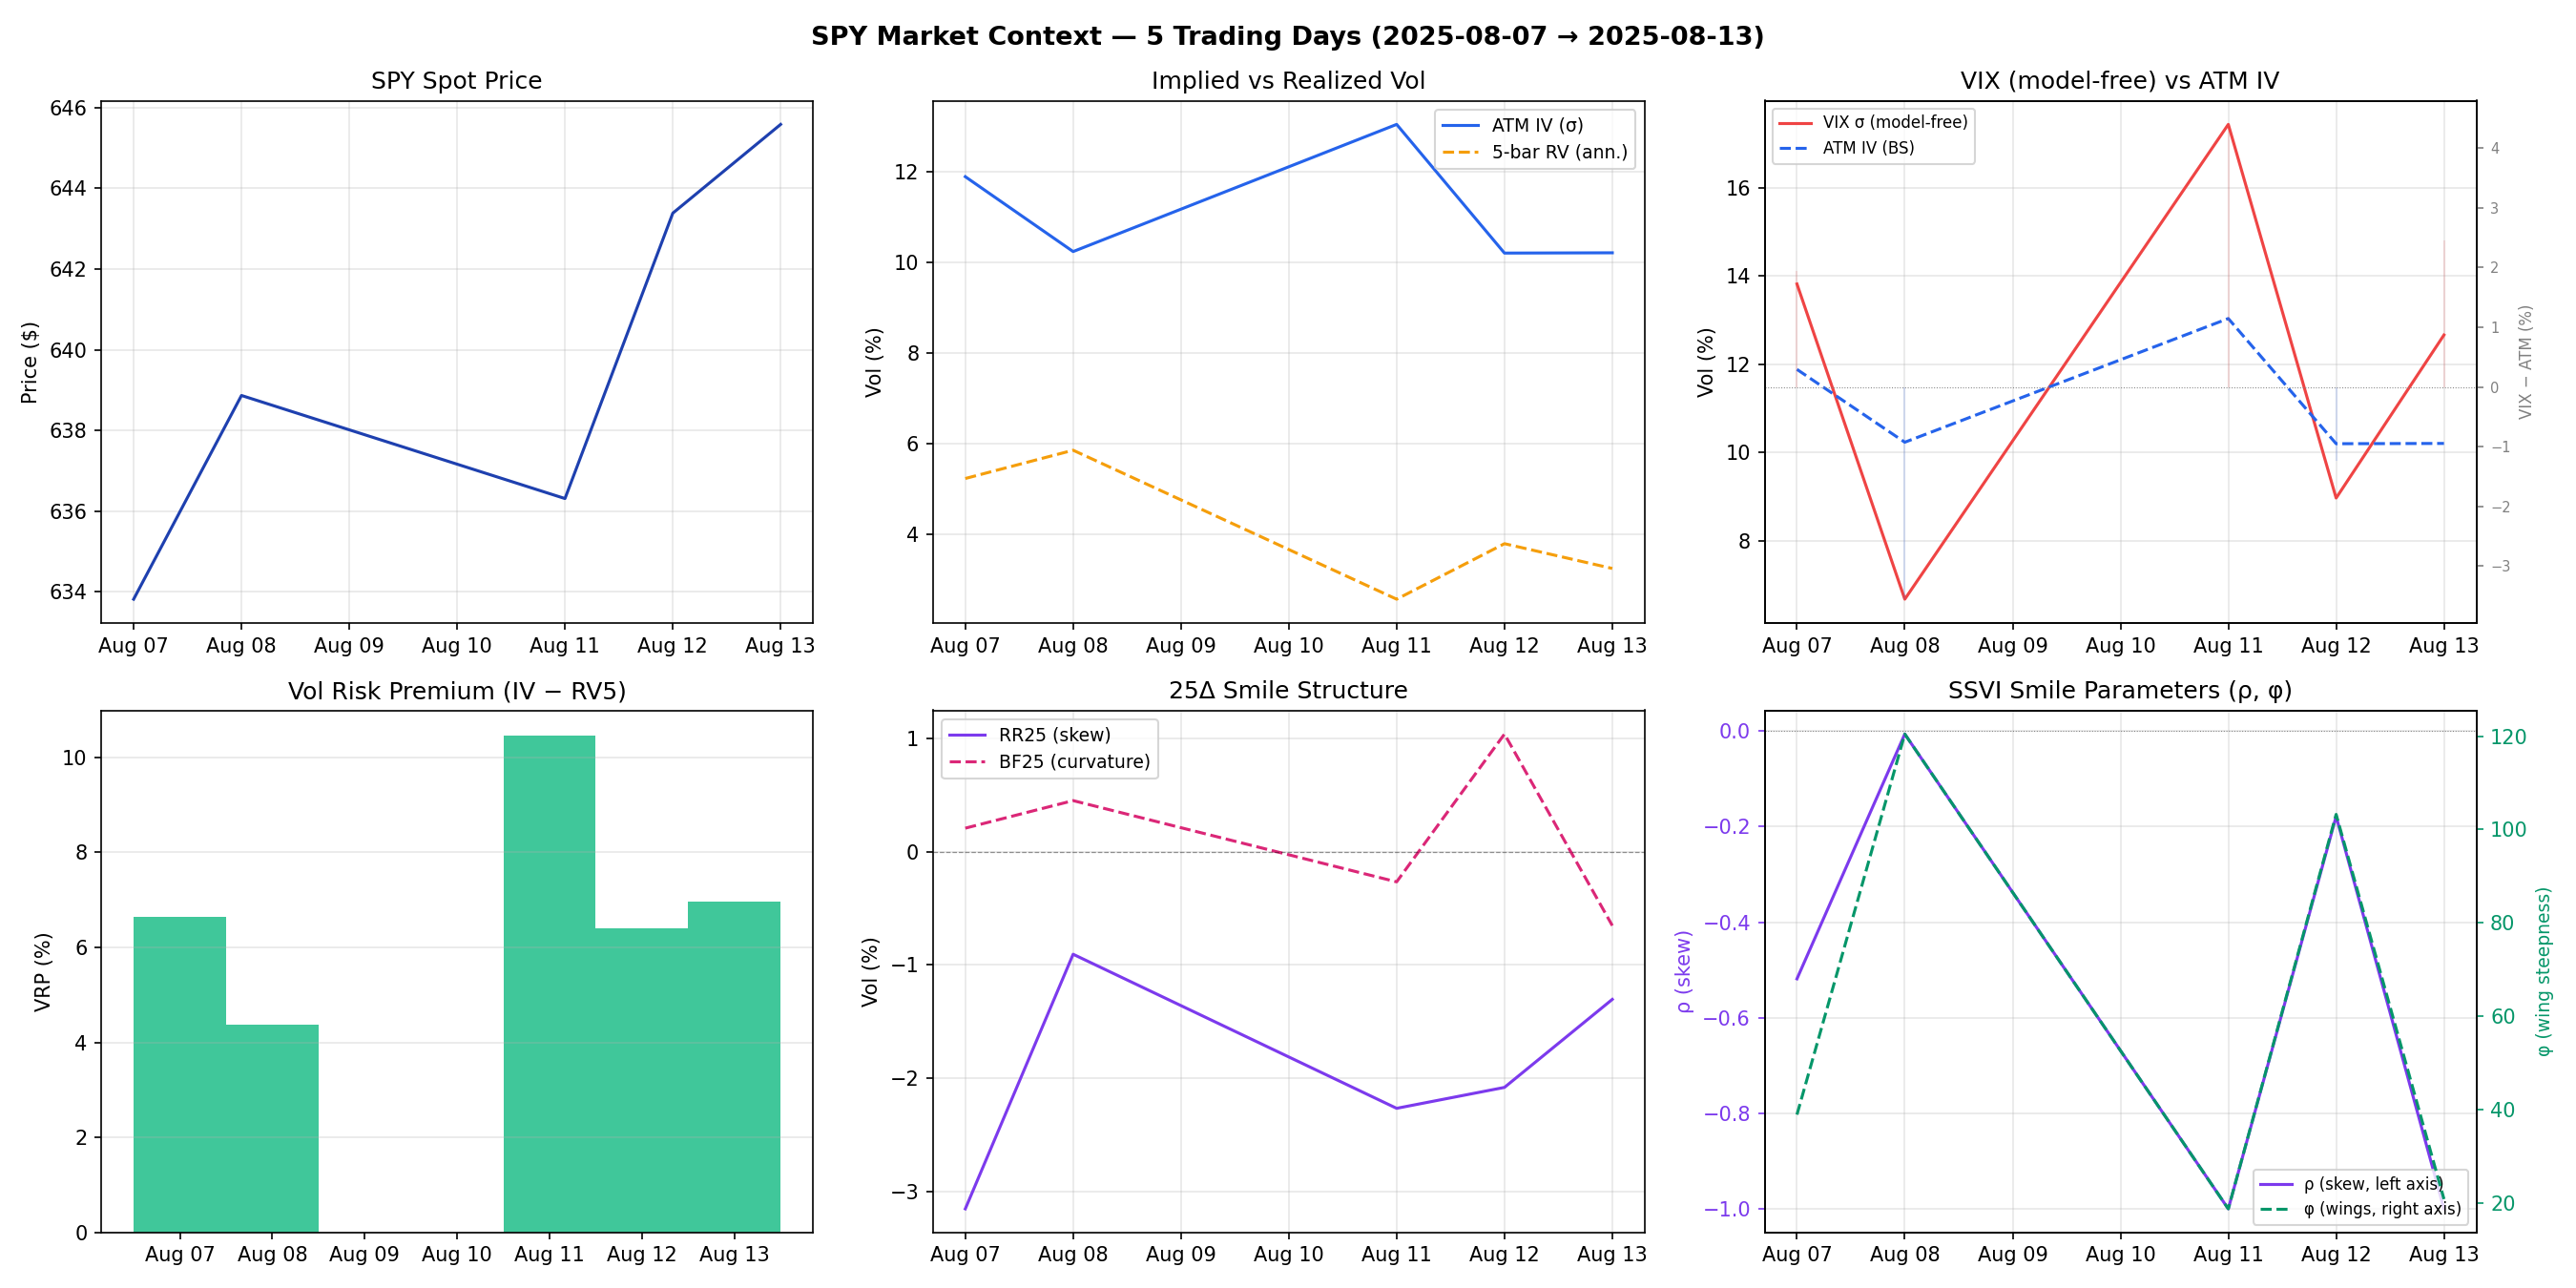
\includegraphics[width=0.92\linewidth,height=0.78\textheight,keepaspectratio]{fig2_market_context.png}
    \vspace{2pt}

    \scriptsize
    The dashboard tracks spot, ATM IV, realized vol, model-free VIX variance, 25$\Delta$ smile structure, and SSVI dynamics.
\end{frame}

% =========================================================
\section{Hedging Models}
% =========================================================

\begin{frame}{PnL Anatomy: Alpha Versus Hedge}
    \small
    \begin{block}{Delta-hedged option PnL, schematically}
    \[
        \dd \Pi_t
        \approx
        \underbrace{\Delta_t \dd S_t}_{\text{spot}}
        +
        \underbrace{\frac12 \Gamma_t \dd \langle S\rangle_t}_{\text{gamma / realized variance}}
        +
        \underbrace{\nu_t \dd \sigma_t}_{\text{vega / surface move}}
        +
        \underbrace{\Theta_t \dd t}_{\text{decay}}
        -
        \mathrm{costs}.
    \]
    \end{block}
    \begin{itemize}
        \item The hedge should remove unwanted spot exposure.
        \item It should \claim{not automatically remove} the gamma/vega residual that carries the volatility premium.
        \item This is why the hedging objective is a strategic choice, not only a modeling detail.
    \end{itemize}
\end{frame}

\begin{frame}{Four Hedgers Tested}
    \small
    \begin{center}
    \renewcommand{\arraystretch}{1.18}
    \begin{tabular}{p{0.22\textwidth}p{0.60\textwidth}}
    \toprule
    \textbf{Hedger} & \textbf{Delta computation} \\
    \midrule
    BSDelta & $N(d_1)$ at market ATM IV and historical time-to-expiry. \\
    RoughVolDelta & BS delta plus Bergomi--Guyon smile-slope correction. \\
    NeuralBSDE-Full & ONNX network trained to replicate the full discounted payoff. \\
    NeuralBSDE-Delta & ONNX network trained to replicate only BS delta hedge PnL. \\
    \bottomrule
    \end{tabular}
    \end{center}
    \vspace{4pt}
    \begin{alertblock}{Hypothesis}
    A neural hedge can be useful only if its training target matches the trading objective.
    \end{alertblock}
\end{frame}

\begin{frame}{Rough Volatility: Why It Enters}
    \small
    \begin{columns}[T,onlytextwidth]
    \begin{column}{0.52\textwidth}
    \begin{block}{State variable}
    \[
    X_t =
    \bigl(\tau,\log(S/K),V_t,U_1,U_2,U_3,U_4\bigr).
    \]
    \end{block}
    \begin{itemize}
        \item Rough-vol models capture short-time skew scaling.
        \item Four OU factors approximate the rough kernel in Markovian form.
        \item The network input is 7D, already beyond comfortable finite-difference grids.
    \end{itemize}
    \end{column}
    \begin{column}{0.42\textwidth}
    \begin{block}{Rough delta correction}
    \[
        \Delta_{\mathrm{rough}}
        =
        \Delta_{\mathrm{BS}}
        +
        \mathrm{Vega}
        \cdot
        \frac{\partial \sigma_K}{\partial S}.
    \]
    \end{block}
    \begin{itemize}
        \item More complete hedge.
        \item But it can consume carry in a positive-VRP regime.
    \end{itemize}
    \end{column}
    \end{columns}
\end{frame}

\begin{frame}{Deep BSDE Hedging: The Modeling Bridge}
    \small
    \begin{block}{Zero-driver BSDE recursion}
    \[
        Y_{t+\Delta t}
        =
        Y_t
        +
        Z_t \cdot \Delta W_t,
        \qquad
        Y_T=\Phi(X_T).
    \]
    \end{block}
    \begin{itemize}
        \item By Feynman--Kac, $Y_t=u(t,X_t)$ and $Z_t$ is the Brownian hedge exposure.
        \item A shared-weight MLP maps each normalized state to $(Y,Z)$.
        \item Export to ONNX makes the hedge available inside the C++ replay loop.
    \end{itemize}
    \vspace{2pt}
    \begin{center}
    \begin{tabular}{ll}
    \toprule
    \textbf{Training mode} & \textbf{Economic meaning} \\
    \midrule
    \texttt{lrh} & Full payoff replication; removes nearly all residual alpha. \\
    \texttt{lrh\_delta} & Delta-only target; leaves gamma + vega as VRP exposure. \\
    \bottomrule
    \end{tabular}
    \end{center}
\end{frame}

\begin{frame}{The Key Discovery: Full Replication Can Kill Alpha}
    \small
    \begin{columns}[T,onlytextwidth]
    \begin{column}{0.47\textwidth}
    \begin{block}{Full replication target}
    \[
        Y_0+\sum_i Z_i\Delta W_i
        \approx
        e^{-rT}(S_T-K)^+.
    \]
    \end{block}
    \begin{itemize}
        \item The model learns to neutralize payoff risk.
        \item That includes the gamma/vega residual that the variance strategy wants.
    \end{itemize}
    \end{column}
    \begin{column}{0.47\textwidth}
    \begin{alertblock}{Delta-only target}
    \[
        \Phi_{\Delta}
        =
        \sum_i N(d_{1,i})\,
        \sigma_i S_i\,
        \Delta W_i.
    \]
    \end{alertblock}
    \begin{itemize}
        \item The model learns the hedge component.
        \item The residual $\Gamma+\nu$ remains available as alpha.
    \end{itemize}
    \end{column}
    \end{columns}
\end{frame}

% =========================================================
\section{System Architecture}
% =========================================================

\begin{frame}{C++ Event-Driven Replay Architecture}
\centering
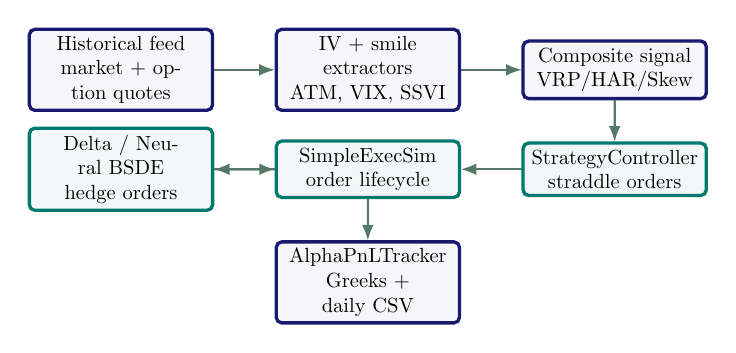
\begin{tikzpicture}[
    scale=0.74,
    transform shape,
    node distance=0.62cm,
    box/.style={draw=midnightblue, rounded corners=2pt, very thick, align=center,
        minimum height=0.62cm, text width=0.24\textwidth, fill=midnightblue!4},
    gbox/.style={draw=pinegreen, rounded corners=2pt, very thick, align=center,
        minimum height=0.62cm, text width=0.24\textwidth, fill=pinegreen!5},
    arrow/.style={-{Latex[length=2mm]}, thick, draw=graygreen}
]
\node[box] (feed) {Historical feed\\market + option quotes};
\node[box, right=1.05cm of feed] (extract) {IV + smile extractors\\ATM, VIX, SSVI};
\node[box, right=1.05cm of extract] (signal) {Composite signal\\VRP/HAR/Skew};
\node[gbox, below=0.72cm of signal] (controller) {StrategyController\\straddle orders};
\node[gbox, left=1.05cm of controller] (exec) {SimpleExecSim\\order lifecycle};
\node[gbox, left=1.05cm of exec] (hedge) {Delta / Neural BSDE\\hedge orders};
\node[box, below=0.72cm of exec] (pnl) {AlphaPnLTracker\\Greeks + daily CSV};
\draw[arrow] (feed) -- (extract);
\draw[arrow] (extract) -- (signal);
\draw[arrow] (signal) -- (controller);
\draw[arrow] (controller) -- (exec);
\draw[arrow] (exec) -- (hedge);
\draw[arrow] (hedge) -- (exec);
\draw[arrow] (exec) -- (pnl);
\end{tikzpicture}
\vspace{5pt}

\scriptsize
The C++ side is deliberately close to production semantics: events, fills, provenance, risk controls, and replayable PnL.
\end{frame}

\begin{frame}{Execution Layer v2: Why It Matters}
    \small
    \begin{center}
    \renewcommand{\arraystretch}{1.18}
    \begin{tabular}{p{0.25\textwidth}p{0.31\textwidth}p{0.31\textwidth}}
    \toprule
    \textbf{Area} & \textbf{Before} & \textbf{Now} \\
    \midrule
    Hedge fills & Hedgers could self-fill and update positions. & Hedgers submit orders; execution publishes fills. \\
    Provenance & Alpha and hedge fills could blur. & Orders/fills carry producer and order id. \\
    Lifecycle & One-shot fill assumption. & Accepted, rejected, partial, filled, canceled reports. \\
    Risk gates & Mostly logging. & Block, cancel, and reduce-only behavior in router. \\
    Accounting & Position updates could precede execution. & Positions update only from execution fills. \\
    \bottomrule
    \end{tabular}
    \end{center}
    \begin{alertblock}{Research implication}
    Once execution is explicit, turnover and transaction costs become model-selection criteria.
    \end{alertblock}
\end{frame}

\begin{frame}{Walk-Forward Retraining Is Now First-Class}
    \small
    \begin{center}
    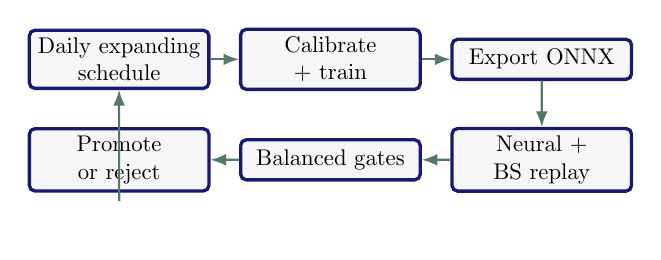
\begin{tikzpicture}[
        scale=0.82,
        transform shape,
        node distance=0.75cm,
        box/.style={draw=midnightblue, rounded corners=2pt, very thick, align=center,
            minimum height=0.62cm, text width=0.21\textwidth, fill=midnightblue!4},
        arrow/.style={-{Latex[length=2mm]}, thick, draw=graygreen}
    ]
    \node[box] (sched) {Daily expanding schedule};
    \node[box, right=0.45cm of sched] (train) {Calibrate + train};
    \node[box, right=0.45cm of train] (export) {Export ONNX};
    \node[box, below=0.72cm of export] (replay) {Neural + BS replay};
    \node[box, left=0.45cm of replay] (gate) {Balanced gates};
    \node[box, left=0.45cm of gate] (promote) {Promote or reject};
    \draw[arrow] (sched) -- (train);
    \draw[arrow] (train) -- (export);
    \draw[arrow] (export) -- (replay);
    \draw[arrow] (replay) -- (gate);
    \draw[arrow] (gate) -- (promote);
    \draw[arrow] (promote) .. controls +(0,-1.1) and +(0,-1.1) .. (sched);
    \end{tikzpicture}
    \end{center}
    \begin{block}{Run layout}
    \texttt{demo/runs/walk\_forward/<run\_id>/windows/<deploy\_date>/}
    stores artifacts, replay CSVs, logs, window manifests, and summary reports.
    \end{block}
\end{frame}

\begin{frame}{Promotion Gates}
    \small
    \begin{center}
    \renewcommand{\arraystretch}{1.18}
    \begin{tabular}{p{0.22\textwidth}p{0.65\textwidth}}
    \toprule
    \textbf{Gate} & \textbf{Checks} \\
    \midrule
    Causality & Train only on rows before deploy date; record train/deploy row counts. \\
    Artifact & Checkpoint, ONNX, normalization, $Y_0$ file, schema, hashes. \\
    ONNX parity & PyTorch versus ONNX output agreement. \\
    Delta sanity & ATM model delta finite and close to BS delta. \\
    Replay health & Neural and BS replays complete and write non-empty daily CSV. \\
    Baseline guard & Neural hedge must not catastrophically underperform BS Delta. \\
    \bottomrule
    \end{tabular}
    \end{center}
    \vspace{2pt}
    \begin{alertblock}{Default behavior}
    No live artifact is overwritten unless all windows pass and \texttt{--promote-if-pass} is explicit.
    \end{alertblock}
\end{frame}

% =========================================================
\section{Results}
% =========================================================

\begin{frame}{OOS Four-Strategy Result}
    \scriptsize
    \begin{center}
    \renewcommand{\arraystretch}{1.15}
    \begin{tabular}{lrrrr}
    \toprule
    \textbf{OOS metric} & \textbf{BSDelta} & \textbf{RoughVol} & \textbf{BSDE-Full} & \textbf{BSDE-Delta} \\
    \midrule
    Hedge PnL & 1,059,605 & 698,612 & 290,817 & 892,723 \\
    Txn cost & 1,801 & 643 & 8,201 & 9,005 \\
    Total PnL & 1,060,036 & 700,201 & 284,847 & 885,950 \\
    vs BSDelta & 100.0\% & 66.0\% & 26.9\% & 83.6\% \\
    \bottomrule
    \end{tabular}
    \end{center}
    \vspace{4pt}
    \begin{block}{Interpretation}
    Full replication is theoretically clean but economically wrong for this alpha; delta-only BSDE keeps most of the variance-premium exposure.
    \end{block}
\end{frame}

\begin{frame}{Cumulative OOS PnL}
    \centering
    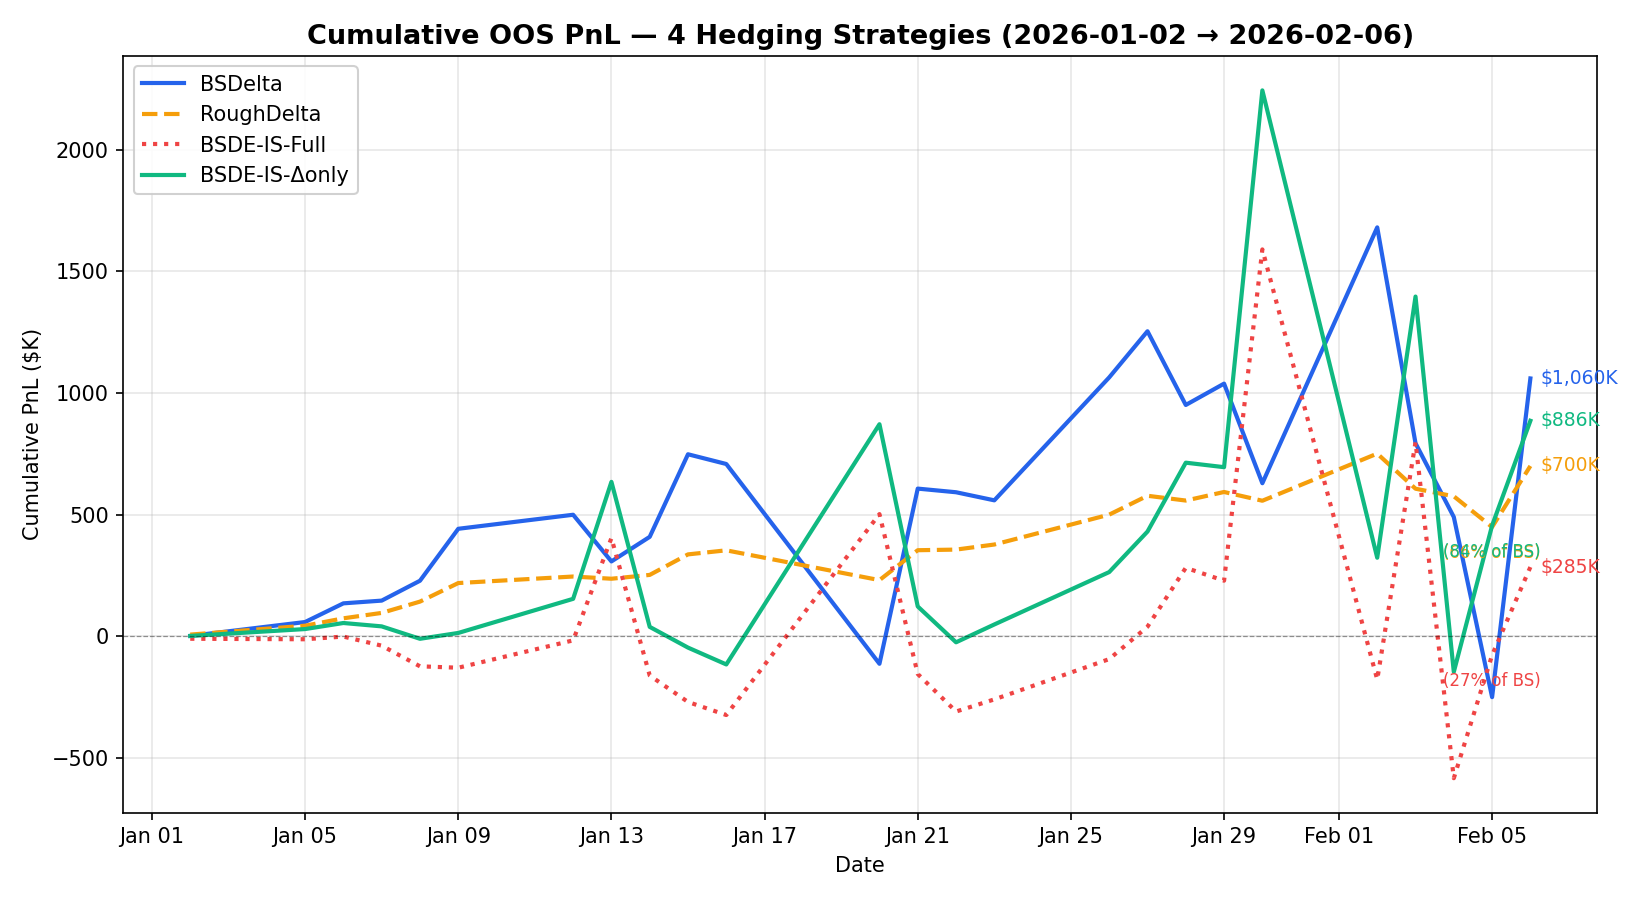
\includegraphics[width=0.92\linewidth,height=0.78\textheight,keepaspectratio]{fig1_cumulative_pnl.png}
    \vspace{2pt}

    \scriptsize
    The delta-only BSDE tracks BSDelta much more closely than the full-replication BSDE.
\end{frame}

\begin{frame}{Greek Attribution Explains The Difference}
    \centering
    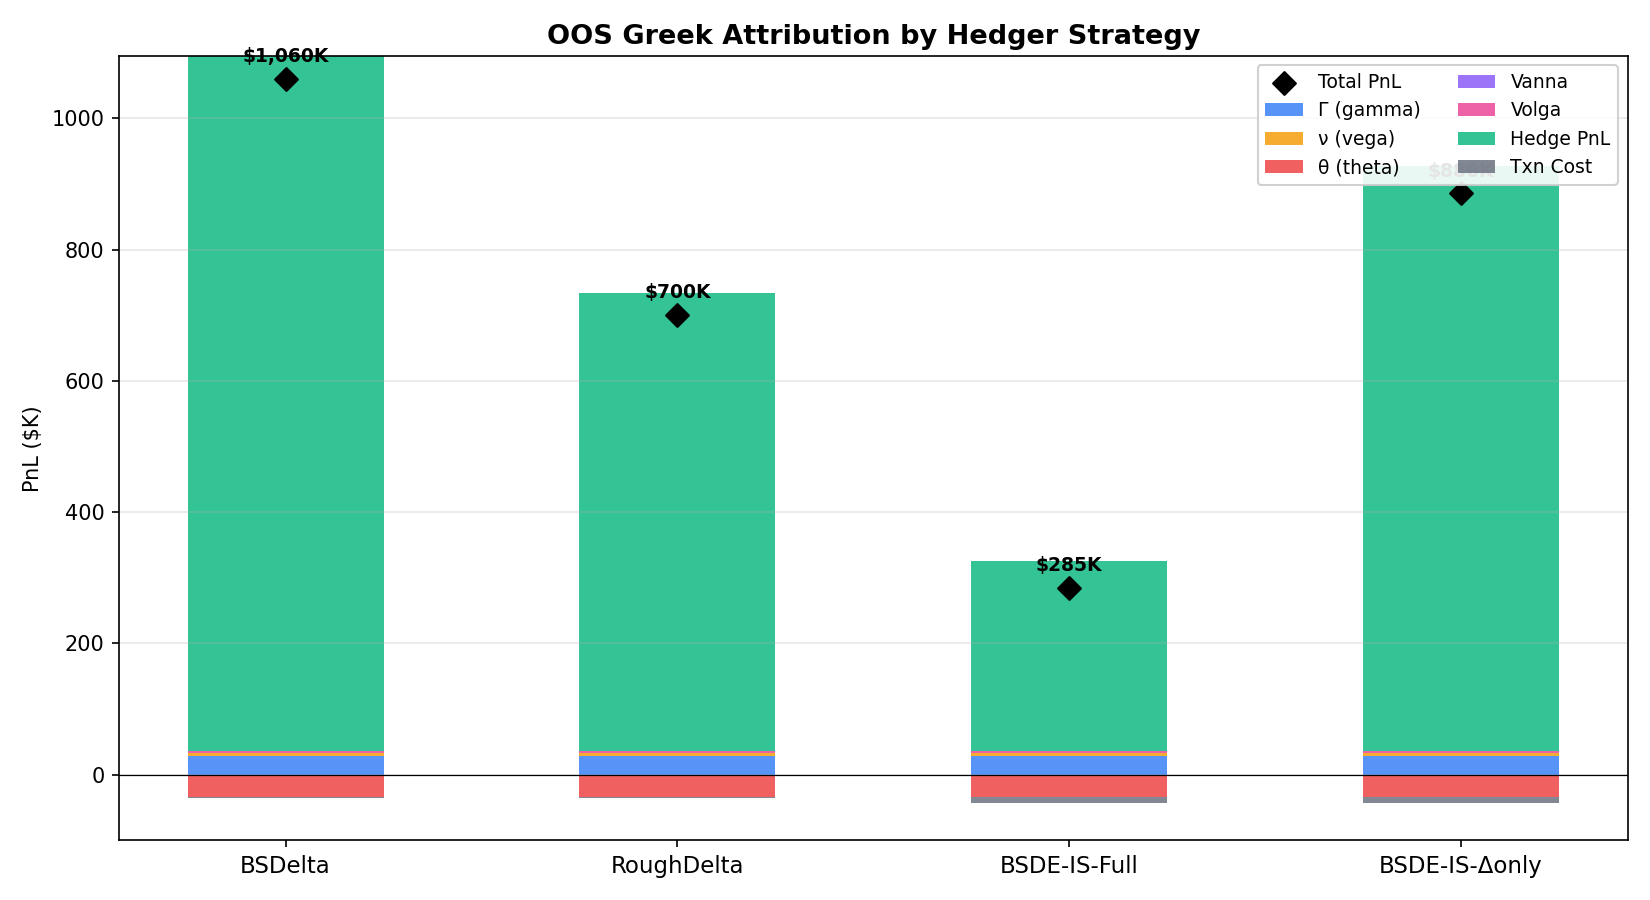
\includegraphics[width=0.92\linewidth,height=0.78\textheight,keepaspectratio]{fig3_greek_attribution.png}
    \vspace{2pt}

    \scriptsize
    Gamma and vega are the intended alpha sources; a hedge objective that erases them also erases the strategy.
\end{frame}

\begin{frame}{Five-Day Walk-Forward Demo Result}
    \small
    \begin{center}
    \renewcommand{\arraystretch}{1.18}
    \begin{tabular}{lr}
    \toprule
    \textbf{Metric} & \textbf{Value} \\
    \midrule
    Total PnL & \$3.415M \\
    Mean daily PnL & \$682,958 $\pm$ \$214,586 \\
    Daily Sharpe & 3.18 \\
    P5 / P50 / P95 & \$311K / \$690K / \$929K \\
    Turnover & 138.8 fills/day \\
    Model delta vs BS & 0.537 vs 0.504 \\
    \bottomrule
    \end{tabular}
    \end{center}
    \begin{alertblock}{Why walk-forward mattered}
    The unretrained synthetic model was out-of-distribution on SPY; SPY calibration fixed the scale of $V_t$, strike, maturity, and skew.
    \end{alertblock}
\end{frame}

\begin{frame}{Daily PnL Stability}
    \centering
    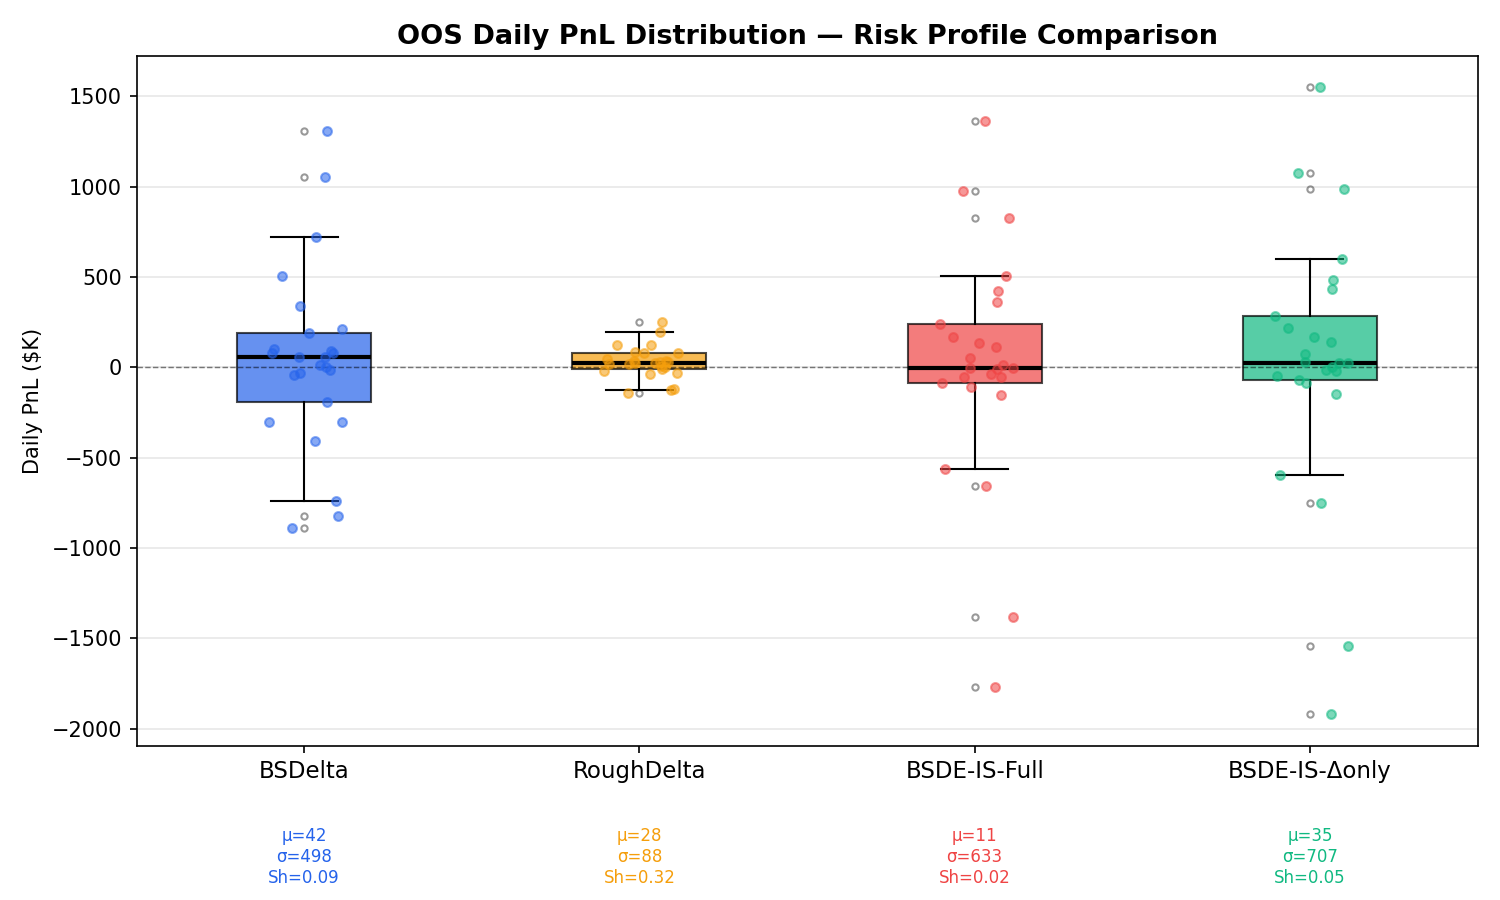
\includegraphics[width=0.90\linewidth,height=0.78\textheight,keepaspectratio]{fig4_daily_distribution.png}
    \vspace{2pt}

    \scriptsize
    The model comparison is not only final PnL; daily dispersion, transaction costs, and residual risk matter.
\end{frame}

% =========================================================
\section{Current Status And Outlook}
% =========================================================

\begin{frame}{What Is Mature Now?}
    \small
    \begin{columns}[T,onlytextwidth]
    \begin{column}{0.48\textwidth}
    \begin{block}{Solid prototype pieces}
    \begin{itemize}
        \item Event-driven C++ replay path.
        \item Multi-strategy hedge comparison.
        \item Greek attribution and daily CSV output.
        \item ONNX inference inside replay.
        \item Walk-forward run manifests and gates.
    \end{itemize}
    \end{block}
    \end{column}
    \begin{column}{0.48\textwidth}
    \begin{alertblock}{Still research-grade}
    \begin{itemize}
        \item Small public/local panel in the repo.
        \item No live broker connectivity.
        \item Simplified execution simulator.
        \item BSDE objective still needs broader regime validation.
        \item Risk sizing and portfolio construction remain MVP-level.
    \end{itemize}
    \end{alertblock}
    \end{column}
    \end{columns}
\end{frame}

\begin{frame}{Main Limitations}
    \small
    \begin{itemize}
        \item \claim{Data scale:} the research claim needs more dates, more regimes, and stricter OOS splits.
        \item \claim{Cost model:} current fills are replay-realistic but not yet venue/microstructure-realistic.
        \item \claim{Model objective:} delta-only works better here, but it should be stress-tested against alternative hedge losses and residual-risk metrics.
        \item \claim{Rough state inference:} U-factors are retained but zeroed at inference to avoid learned confounds.
        \item \claim{Promotion policy:} gates exist, but production would need monitoring, rollback, and capital/risk budgets.
    \end{itemize}
\end{frame}

\begin{frame}{Roadmap}
    \small
    \begin{center}
    \renewcommand{\arraystretch}{1.18}
    \begin{tabular}{p{0.20\textwidth}p{0.66\textwidth}}
    \toprule
    \textbf{Next step} & \textbf{Goal} \\
    \midrule
    More data regimes & Test positive VRP, negative VRP, stress, quiet, high-rate, low-rate windows. \\
    Better replay costs & Add latency, queue position, venue fee model, and spread impact. \\
    Residual-risk gate & Evaluate hedge residual variance, not only total PnL. \\
    Objective sweep & Compare full payoff, delta-only, residual variance, and transaction-cost-aware losses. \\
    Portfolio layer & Move from one straddle engine to risk-budgeted multi-expiry/multi-strike books. \\
    \bottomrule
    \end{tabular}
    \end{center}
\end{frame}

\begin{frame}{Takeaway}
    \small
    \begin{center}
    \begin{minipage}{0.82\textwidth}
    \begin{block}{Main message}
    The project's major idea is that a neural BSDE should be used as a \claim{hedging operator} inside a full trading system, not as an isolated pricing model.
    \end{block}
    \vspace{5pt}
    For volatility alpha, the right question is:
    \[
        \text{Which risks should the model hedge, and which residuals are the alpha?}
    \]
    The current evidence says full replication can destroy the variance premium, while a delta-only BSDE preserves most of the exposure and can be deployed through a gated walk-forward pipeline.
    \end{minipage}
    \end{center}
\end{frame}

\begin{frame}
    \vspace{30pt}
    \begin{center}
        {\Huge \color{midnightblue} \textbf{Thank You}}

        \vspace{20pt}
        {\large \textbf{Questions \& Discussion}}

        \vspace{14pt}
        {\small \texttt{Effective Engine MVP}}
    \end{center}
\end{frame}

\appendix
\section*{References}
\begin{frame}[allowframebreaks]{References}
    \scriptsize
    \bibliographystyle{alphaurl}
    \bibliography{references}
\end{frame}

\end{document}
